% !TEX encoding = UTF-8 Unicode
% !TEX root = BioInspired.tex

%%%  This is the main driver file.   It is mostly a list of file includes.   Read through and edit as needed.

\documentclass[table]{book}

\usepackage{listings}
\usepackage{color}

\definecolor{dkgreen}{rgb}{0,0.6,0}
\definecolor{gray}{rgb}{0.5,0.5,0.5}
\definecolor{mauve}{rgb}{0.58,0,0.82}

\lstset{frame=tb,
  language=Python,
  aboveskip=3mm,
  belowskip=3mm,
  showstringspaces=false,
  columns=flexible,
  basicstyle={\small\ttfamily},
  numbers=none,
  numberstyle=\tiny\color{gray},
  keywordstyle=\color{blue},
  commentstyle=\color{dkgreen},
  stringstyle=\color{mauve},
  breaklines=true,
  breakatwhitespace=true,
  tabsize=3
}

\usepackage[width=6.5in, height=9.0in, top=1.0in, papersize={8.5in,11in}]{geometry}
\usepackage[pdftex]{graphicx}
\DeclareGraphicsExtensions{.pdf,.png,.jpg}
%\usepackage{draftwatermark}
\usepackage{amsmath}
\usepackage{amsthm}
\usepackage{amssymb}
%\usepackage{txfonts}
\usepackage{textcomp}
%\usepackage{amsthm}
%\usepackage{array}
%\usepackage{datetime}
\usepackage{anyfontsize}
\usepackage{t1enc}
\usepackage[section,subsection]{extraplaceins}   %%%  \FloatBarrier
\usepackage[all]{xy}
\usepackage{fancyhdr}
\usepackage{hyperref}
\usepackage{verbatim}
\usepackage{algorithm}
\usepackage{makeidx}
\usepackage{multicol}
\usepackage{multirow}
\usepackage{color}
\usepackage{rotating}
\usepackage{wrapfig}
\usepackage{tikz}
\usetikzlibrary{shapes.geometric, arrows}
%\usepackage{tabularx}
\usepackage{xcolor}
\usepackage{framed}
\usepackage{xspace}
\usepackage{listings}
\lstset{language=python,frame=ltrb,framesep=5pt,basicstyle=\normalsize,
 keywordstyle=\ttfamily\color{DarkRed},
%morecomment=[n][\textbf]{In\ [}{]\:},
%morecomment=[n][\textbf]{Out\ [}{]\:},
morecomment=[s][\color{blue}]{In\ [}{]\:},
morecomment=[s][\color{red}]{Out[}{]\:},
identifierstyle=\ttfamily\color{DarkBlue}\bfseries,
commentstyle=\color{OliveGreen},
stringstyle=\ttfamily,
showstringspaces=false,tabsize = 3}

\lstdefinelanguage{shell} {
commentstyle = \color{black},
keywordstyle = \color{black},
stringstyle = \color{black},
identifierstyle = \color{black},
morecomment=[s][\color{blue}]{In\ [}{]\:},
morecomment=[s][\color{red}]{Out[}{]\:},
 }

\newtheorem{thrm}{Theorem}
\newtheorem{lem}[thrm]{Lemma}
\newtheorem{cor}[thrm]{Corollary}
\newtheorem{rem}[thrm]{Remark}
\newtheorem{defn}[thrm]{Definition}
\newtheorem{exmpl}[thrm]{Example}

% this gives a little box for the end of a proof:
%
\def\endthrmbox{$\sqsubset \!\!\!\! \sqsupset$}

\newcommand{\dis}{\displaystyle}
 \def      \RR             {{\mathbb R}} 
        \def      \NN             {{\Bbb N}} 
        \def      \QQ             {{\Bbb Q}} 
        \def      \CC             {{\Bbb C}} 
        \def      \ZZ             {{\Bbb Z}} 
 
 
        \def       \a              {{\alpha}} 
        \def       \b              {{\beta}} 
        \def       \d              {{\delta}} 
        \def       \D              {{\Delta}} 
        \def         \e              {{\varepsilon}} 
        \def         \g              {{\gamma}} 
        \def         \G              {{\Gamma}} 
        \def       \l              {{\lambda}} 
        \def       \L              {{\Lambda}} 
        \def        \m               {{\mu}} 
        \def         \n              {{\nabla}} 
        \def       \var          {{\varphi}} 
        \def         \s              {{\sigma}} 
        \def       \Sig          {{\Sigma}} 
        \def       \Om          {{\Omega}} 
 
        \def       \t              {{\tau}} 
        \def         \th             {{\theta}} 
        \def       \O              {{\Omega}} 
        \def       \o              {{\omega}} 
        \def         \z              {{\zeta}} 
       \def        \P             {{\Phi}} 
       \def        \p             {{\phi}} 
        %Other macros 
 
        \def       \iy              {{\infty}} 
        \def         \pa             {{\partial}} 
        \def         \div           {{\rm div}} 
         \def       \na            {{\nabla}} 
 



\newcommand{\pythonlogo}{
\\[-2mm] \begin{picture}(0,0)
\put(-40,-40){\includegraphics[scale=0.25]{./Figures/pythonlogo.png}}
\end{picture}
}

\newcommand{\clogo}{
\\[-2mm] \begin{picture}(0,0)
\put(-30,-30){\includegraphics[scale=0.2]{./Figures/clogo.png}}
\end{picture}
}

\newcommand{\roslogo}{
\\[-2mm] 
\begin{picture}(0,0)
\put(-30,-30){\includegraphics[scale=0.2]{./Figures/roslogo.png}}
\end{picture}
}


\tikzstyle{master} = [rectangle, draw, text width=6em, text centered, minimum
height=3em]
\tikzstyle{node} = [rectangle, draw, text width=6em, text centered, rounded
corners, minimum height=3em]

\newtheorem{summary}{Summary:}
\newtheorem{example}{Example:}[section]

\definecolor{OliveGreen}{cmyk}{0.64,0,0.95,0.40}
\definecolor{DarkBlue}{cmyk}{0.76,0.76,0,0.20}
\definecolor{DarkRed}{cmyk}{0,1,1,0.45}


\def      \RR             {{\mathbb R}} 
\def      \DS            {\displaystyle} 

\setlength{\oddsidemargin}{0mm} 
\setlength{\evensidemargin}{0mm} 

%\SetWatermarkLightness{0.975}
%\SetWatermarkScale{6}
%\SetWatermarkText{\includegraphics{test.png}}

\pagestyle{fancy}
\renewcommand{\chaptermark}[1]{\markboth{#1}{}}
\renewcommand{\sectionmark}[1]{\markright{\thesection\ #1}}
\fancyhf{}
\fancyhead[LE,RO]{\bfseries\thepage}
\fancyhead[LO]{\bfseries\rightmark}
\fancyhead[RE]{\bfseries\leftmark}
\renewcommand{\headrulewidth}{0.5pt}
\renewcommand{\footrulewidth}{0pt}
\addtolength{\headheight}{0.5pt}
\setlength{\footskip}{0in}
\renewcommand{\footruleskip}{0pt}
\fancypagestyle{plain}{%
\fancyhead{}
\renewcommand{\headrulewidth}{0pt}
}


\definecolor{color02}{rgb}{0.18,0.35,0.59}
\definecolor{color03}{rgb}{0.44,0.59,0.82}
\definecolor{color06}{rgb}{0.35,0.35,0.35}


\definecolor{MSBlue}{rgb}{.204,.353,.541}
\definecolor{MSLightBlue}{rgb}{.31,.506,.741}
\definecolor{MSBlue1}{rgb}{0.18,0.35,0.59}
\definecolor{MSBlue2}{rgb}{0.44,0.59,0.82}
\definecolor{MSBlue3}{rgb}{0.35,0.35,0.35}

\usepackage{titlesec}
\titleformat{\chapter}[display]
%{\normalfont\bfseries\color{MSBlue1}}    %\normalfont\bfseries\filcenter}
{\normalfont\bfseries}    %\normalfont\bfseries\filcenter}
{\LARGE\thechapter}
{1ex}
{\titlerule[2pt]
\vspace{2ex}%
\LARGE}
[\vspace{1ex}%
{\titlerule[2pt]}]



\date{\today}

 % This sets the format.

% Add your title page contents here 
\title{{ \rule{\linewidth}{0.5mm}}\\[2mm] {\huge \bfseries  CSC 492/592 BioInspired Computing }\\[-1mm] {\rule{\linewidth}{0.5mm}} \\  \vfill
{\LARGE \bfseries  Homework 2 }\vfill}
\author{Ian Carlson \and  Derek Stotz  }
\date{\today}


\begin{document}

\frontmatter

% Comment out items you don't need

\addcontentsline{toc}{chapter}{Title}
\maketitle
\tableofcontents
\addcontentsline{toc}{chapter}{Contents}
\listoffigures
\addcontentsline{toc}{chapter}{List of Figures}
\listoftables
\addcontentsline{toc}{chapter}{List of Tables}

\chapter{Document Preparation and Updates}
% !TEX root = BioInspired.tex



Current Version [1.0.0]
\vspace*{5mm}

{\color{MSBlue3}
\noindent
\textit{Prepared By:}\\
\textit{Mack Smith}\\
\textit{Derek Stoz}
}

\vfill
\noindent
{\color{color02} \textit{\textbf{Revision History}}}\\
\begin{tabular}{|>{\raggedright}p{1.5cm}|>{\raggedright}p{3cm}|>{\raggedright}p{1.5cm}|>{\raggedright}p{9cm}|}
\hline
\textit{\textbf{Date}} &  \textit{\textbf{Author}} & \textit{\textbf{Version}} & \textit{\textbf{Comments}}\tabularnewline
\hline
 \textit{\textbf{5/2/15}} & \textit{Mack Smith and Derek Stoz} & \textit{1.0.0} & \textit{Finished all programs and some portions of documentation}\tabularnewline
\hline
 \textit{\textbf{5/4/15}} & \textit{Mack Smith and Derek Stoz} & \textit{1.0.0} & \textit{Wrote the rest of the documentation}\tabularnewline
 \hline
 &  &  & \tabularnewline
\hline
 &  &  & \tabularnewline
\hline
 &  &  & \tabularnewline
\hline
 &  &  & \tabularnewline
\hline
\end{tabular}
\vfill


 
 % Core content to follow ...
 
\mainmatter

%%  Add to the following chapters
% you may also need additional chapters ...

% !TEX root = BioInspired.tex

\chapter{Evolutionary Algorithms - Text Chapter 3}

\section{Problem 3.1 and 3.2}
Implement the various hill-climbing procedures and the simulated annealing algorithm to solve the problem exemplified in Section 3.3.3. use a real-valued representation scheme for the candidtate solutions (variable x). By comparing the performance of the algorithms, what can you conclude?

For 3.2, also implement an genetic algorithm to do the same.

For the simple hill climbing, try different initial configurations as attempts at finding the global optimum. Was this algorithm succesful?

Discuss the sensitivity of the algorithms in relations to their input parameters.

\subsection{Problem Information}

The goal of the problem in 3.3.3 referenced by the text was to find the global maximum of the equation $g(x) = 2^{-2(\frac{x-.1}{.9})^2}sin(5\pi x)^6$. By inspection of the graph given in the textbook, we know that the optimal x value is 0.1, and the global maximum is 1. All algorithms were evaluated by whether or not they reliably converged to this answer.

\subsection{Deterministic Hill Climb}

\subsubsection{Algorithm Description}
The first algorithm we implemented was the deterministic hill climb. In this program, we chose a random starting x value, and input a fixed number of time-steps. At each time-step, the algorithm checks to the left and right of the current position by a fixed step-size. If a better solution is found, the algorithm moves one step in that direction. This repeats until no improvement can be made, or the maximum number of iterations is reached.

\subsubsection{Algorithm Performance}
This algorithm, in general, was not succesful. Even when the starting domain was restricted between -1 and 1, the algorithm only converged to the global maximumin  approximately 10\% of the trials. In the other 90\% of the trials, the starting x value was outside the "hill" of the global maximum, and it would converge to to a local maximum instead.

\subsubsection{Sensitivity}
We considered the sensitiviy of the algorithm to 3 input parameters: starting x value, step size, and number of time steps.

This method is extremely sensitive to the starting x value. If there is not a monotonicaly increasing slope from the starting value to the global maximum, deterministic hill climb will not find it. This algorithm does, however, always find the nearest local maximum, and does so very quickly.

The resolution of the final result depends on the step size, but as long as the step size is reasonably small it does not effect whether or not the algorithm will converge on a local maximum.

The final result is sensitive to the maximum number of iterations. If the distance between the starting x value and the x value of the local maximum is greater than the number of iterations multiplied by the step-size, the local maximum will not be reached when the program terminates.

\subsection{Stochastic Hill Climb}

\subsubsection{Algorithm Description}
The stochastic hill climb was a slight variation on the deterministic hill climb. Instead of looking left and right by a fixed step size, we instead would pick a random floating point number from a uniform distribution between -p and p, where p was one of our input parameters. At each time step, we would generate this random number and add it to the current x value. If the new location had a higher fitness than the old location, we would replace the current x value with that new x value. This algorithm terminated once the maximum number of iterations was reached, or if the fitness of the current x value was equal to the global maximum, which we knew to be 1 by examination of the graph of the function.

\subsubsection{Algorithm Performance}
This algorithm was hit and miss and highly sensitive to paramters, as will be discussed in the next section. In general, this algorithm performed better than the deterministic hill climb because it had the potential to jump out of local maxima. However, it also had the potential to jump away from the global maximum rather than converging.

For this particular problem, we were able to find a set of parameters that nearly always converged to the global maximum in the time allowed, but from a computational perspective, it wasn't much better than random search.

\subsubsection{Sensitivity}
We analyzed three input parameters: starting x value, perturbation size - referred to as p above, and maximum number of iterations.

The starting x value had some impact on whether the algorithm would converge, but not nearly as much as in the deterministic version because the algorithm had the potential to jump out of local maxima in favor of maxima with higher fitness. Of course, if the starting x value was randomly generated very close to the global maximum, it nearly guaranteed the algorithm would converge to the global maximum.

The most important parameter was the perturbation size. A very large perturbation allowed the algorithm to jump out of local maxima much more frequently, but it also took much longer to converge to any maxima, and may not converge at all if the maximum number of iterations was too small. If the perturbation size was very small, the algorithm would quickly converge on a maxima, but be unable to jump out of local maxima. The proper value for this parameter seems to be highly problem dependant, and is affected by the maximum allowable number of iterations. If an infinite number of iterations were allowed, having a very large perturbation size would be allowable. The algorithm may jump between maxima with a high frequency, but the algorithm never chooses a new x value with a lower fitness than the current one, so it would eventually find the global maximum.

The maximum number of iterations on its own had little effect on the final solution except in the case noted in the discussion about perturbation size.

\subsection{Shotgun Hill Climb}

\subsubsection{Algorithm Description}

This algorithm is also known as iterated hill climb in the text, but we liked the Wikipedia name a little better. The basic premise of shotgun hill climb is to run a hill  climb algorithm many times with different starting positions, and keep track of the best of all runs. For this particular problem, we chose to iteratively apply the stochastic hill climbing method. Since the stochastic hill climb nearly always converged, applying it with many different starting x values basically guaranteed convergence. In our application, we chose the starting x value randomly for each iteration, but another method would be to uniformly sample the feature space.

\subsubsection{Algorithm Performance}

This algorithm worked very well. For this problem, it might be the fastest and most reliable solution. However, for problems with very large and complex feature spaces, fully sampling the space might not be desirable or even possible. At the very least it is an easy first attempt for finding a least a very good local maximum of a complex feature space.

\subsubsection{Sensitivity}

The most interesting feature of the shotgun hill climb is its insensitivity to starting parameters. Even if the hill climb algorithm were set up with poor starting conditions or input parameters, applying the algorithm multiple times typically still manages to force convergence to a solution. We purposefully chose input parameters that caused poor performance with our stochastic hill climb, but the shotgun hill climb still converged to the global maximum every time we ran it.

\subsection{Simulated Annealing}

\subsubsection{Algorithm Description}

Simulated annealing attempts to combine the ability of the stochastic hill climb to jump out of local maxima with the high probability of convergence on a given maxima of the deterministic hill climb. The primary feature is the introduction of the temperature parameter T, which starts out high and diminishes. Much like the stochastic hill climb, a random perturbation is chosen at each time step. However, when T is high, there is a high probability that the algorithm will choose to make the jump even though the fitness at the new location might be lower. As T reduces, it becomes less and less likely that the location will jump to a less fit solution.

\subsubsection{Algorithm Performance}

We had trouble getting the simulated annealing algorithm to converge reliably. This was probably just because we were bad at picking the parameters. This algorithm seems finicky at best, and unreliable at worst.

\subsubsection{Sensitivity}

We analyzed the following paramters: T - the initial temperature, k - the cooling rate, p - perturbation amount. The initial temperature selection seems crucial and very problem specific. In addition, the initial T and the value for k are strongly related. A high T and low k will cause the algorithm to fail to converge in the alotted time. A low T and high k will force the algorithm to end prematurely when T hits near zero. Tuning these two paramters appears complex and more or less trial and error.

\subsection{Simulated Annealing With a Twist}

\subsubsection{Algorithm Description}

We had a thought, when we were having trouble with getting simulated annealing to work, that worked out pretty well so we thought we would include it. In traditional simulated annealing, the probability of accepting a random jump even if it is "worse" than the current location is high when T is high, and decreases as T decreases. Instead, we wrote an algorithm much like the stochastic hill climb, but instead of changing the probability of accepting a jump to a "worse" x value, we changed the size of the allowable jump as T decreased. In other words, when T is high, the perturbations were allowed to be very large. As T diminished, the size of the jumps was reduced and we only accepted a jump when it increased the fitness of the solution. 

\subsubsection{Algorithm Performance}

This performed much better overall than our traditional simulated annealing, as it allowed us to jump out of local maxima with very high frequency at the beginning, but allowed us to converge very accurately to a maxima at the end.

\subsubsection{Sensitivity}

Our modified simulated annealing algorithm seemed much less sensitive to input parameters. However, it did depended on having a high enough initial perturbation size to jump out of local maxima, which is problem specific information. In addition, the rate at which T diminishes appears to have some affect on how likely the algorithm was to get trapped in a local maxima.

\subsection{Evolutionary Algorithm}

\subsubsection{Algorithm Description}

Problem 3.2 requested a Genetic Algorithm for finding the maxizing x for the function $g(x) = 2^{-2(\frac{x-.1}{.9})^2}sin(5\pi x)^6$, where the mutation and crossover was done bitwise.  Implemented in python, this was a new experience for us.  However, the python bitwise operations turned out to be reasonably useable, and using some trickery we were able to find reliable ways to mutate and crossover python's abstract integers.

The starting population filled by generating n numbers between 1 and 0xFFFFFFFF.  When fit, the number is divided and shifted over to reflect a floating point value between -1 and 1.   This allowed us to use bitwise operators to modify representations of floating point values.

The overall algorithm was a traditional GA.  The population was fit by plugging the values into the function, and the results were sorted.  The top [selection rate] percent of "dudes", as we called our individuals, were then bred to create the next population.  Breeding was done by choosing a crossover point in the bit string and copying the left half of one onto the other by means of bitmasking.  Mutation, done [mutation rate] percent of the time after breeding, was done by flipping one random bit in the genome of the dude.

At the end of one generation, the best fit dude was printed and the loop started over again.  After a specified number of iterations, the overall best dude was printed to the screen, showing its fitness and x value.

\subsubsection{Algorithm Performance}

This genetic algorithm performed exceptionally well.  With the default parameters in the code, the best fit dude had a fitness of 1.0 approximately 90\% of the time (or rather, .99999... with too many 9's for python to keep track of).  While the computation time required for such consistently optimal results was much greater than any of the other optimization algorithms applied to this problem, the results were clearly the best.

\subsubsection{Sensitivity}

The genetic algorithm required quite a bit of tweaking in order to settle into finding 1.0 ninety percent of the time.  First of all, increasing the population size greatly stabilized the results, giving more consistently optimal x values in earlier generations.  However, the population size had the greatest effect on performance.  Increasing the maximum generations increased the runtime linearly, but did not always guarantee an eventual convergance.  With our population size of 750, a generation count of 40 seemed to be a sufficiently lengthy lifetime for the program.  The mutation rate, while not really necessary, did lenghen the amount of time that the program deviated before sticking around one fitness value.  Our selection rate was kept low, as we preferred a higher mutation rate as a deviation mechanism for the aforementioned reason.  In addition, a lower selection rate helped keep the runtime low and the results focused on better results.

\section{Problem 3.7}

Determine using genetic programming, the computer program (s-expression) that produces exactly the outputs presented in Table \ref{GP Desired InOut} for each value of x. The following hypotheses are given:

- use only functions with two arguments, i.e. binary trees

- largest depth allowed for each tree: 4

- Function set: \{+,*\}

- Terminal set: T=\{0,1,2,3,4,5,x\}

\begin{table}[tbh]
\caption{Desired Input Output Value Pairs. \label{GP Table}}
\begin{center}
\begin{tabular}{|c|c|c|c|c|c|c|c|c|c|c|c|c|c|c|c|c|c|c|c|c|}
  \hline
-10 & -9 & -8 & -7 & -6 & -5 & -4 & -3 & -2 & -1 & 0 & 1 & 2 & 3 & 4 & 5 & 6 & 7 & 8 & 9 & 10\\
\hline
153 & 120 & 91 & 66 & 45 & 28 & 15 & 6 & 1 & 0 & 3 & 10 & 21 & 36 & 55 & 76 & 105 & 136 & 171& 210 & 253\\
  \hline
\end{tabular}
\end{center}
\end{table}

\subsection{Algorithm Description}

While complex in execution, the approach for solving this problem was simple. An initial set of binary trees $P_O$ was generated, each with one member of the function set (or one nonterminal) as the root, and two members of the terminal set (terminals) as children of the root node. Once the initial population was generated, the following steps were performed in a loop for a fixed number of iterations:

\begin{itemize}
   \item  Evaulate the fitness of each tree
   \item  Sort the trees by fitness
   \item Replace the bottom 50\% using the crossover operation on the top 50\%
   \item Randomly mutate 10\% of the new population
\end{itemize}

While most of the code written was to manage the trees and put together some half-ways readable output, there are a handful of operations worth examining in detail.

\subsubsection{Evaluation}

Evaluation of the fitness of each tree was done by computing the sum of squared differeces between the desired output given in table \ref{GP Table}, and the actual output when a given x value is supplied to the tree. A fitness of 0 was considered optimal.

\subsubsection{Crossover}

Crossover was done by using a roulette style selection to select two parents from the best 50\% of the population. This was done without replacement so one parent could be chosen twice. One parent was randomly selected to be the base parent, and the other the secondary parent. The child was initially created as a clone of the base parent. Then a random node was selected from both the child and the secondary parent. This could be any node, including the root node of either tree. The subtree including the node from the child tree was then replaced with the subtree selected from the secondary parent. If the maximum depth would be violated by this exchange, the nonterminal nodes at the maximum depth were replaced with terminals, and their children were deleted.

\subsubsection{Mutation}

Mutation was done by selecting a random node in the tree, deleting it, and randomly regenerating it. The node selected was determined by picking a random number from a uniform distribution between 0 and $N-1$. The selected node could be any node in the tree, including the root node. If a new node was generated as a nonterminal, the children nodes were also randomly generated. It was therefor possible for a tree to be completely destroyed and randomly rebuilt in a mutation. The probability for this being $\frac{1}{N}$ where $N$ was the number of nodes in the tree. In the random node generation, the maximum depth was enforced by requiring that any node generated on the maximum depth level be generated as a terminal.

\subsubsection{Alternative Mutation}

A second theme for mutation was considered, but not implemented. In this alternative scheme, a node would be selected at random in the tree just like in the method above. However, instead of destroying the node and all of its children (if any), the node's type would remain the same and only the value would change. Hence, nonterminals would remain nonterminals, but the operation could change from + to * or vice versa. Likewise, a terminal would simply change to another terminal value. This idea, while valid, was discarded on the grounds that the method stated above would more thoroughly explore the space by allowing for much more radical changes via mutation.

\subsection{Results}

Running the genetic program with a population of 100 individuals and 3000 generations consistently gives a tree the represents the equation $2x^2 + 5x + 3$ that showed a total sum of squared differences error of 2. We judged this answer against using excell to find a polynomial fit to the given points. Excel gave us the equation $y = 2.001x2 + 4.987x + 2.8666$. Given that we are constrianed to using integer values, this appears to be the optimal achievable solution. There are many different trees that represent the same polynomial, and the algorithm may or may not generate the same one every time. The tree often also contains no-ops, like adding 0, or adding something multiplied by zero because additional nodes do not incurr a fitness penalty. An example run is shown in Figure \ref{fig:gprun}.

\begin{figure}[tbh]
\begin{center}
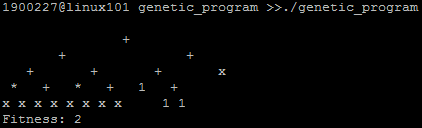
\includegraphics[width=0.75\textwidth]{gprun.png}
\end{center}
\caption{A Sample Genetic Program Run\label{fig:gprun}}
\end{figure}


% !TEX root = BioInspired.tex

\chapter{Text Chapter 4 - Artificial Neural Networks}

\section{Problem 4.17}

Apply the MLP network trained with the backpopagation learning algorithm to solve the character recognition task in 4.4.2.

Determine a suitable network architecture and test the resultant network sensitivity to noise in the test data. Test different noise levels from 5-50\%.

\section{Network Description}

To solve this problem, we implemented a three layer neural network with 120 input nodes, 50 hidden layer nodes, and 8 output nodes. There are 120 input layer nodes so that each pixel has one node. There are 8 output nodes so the network can decide if the test image matches each of the training images independantly. It is entirely possible for the network to match a test image to multiple training images, or none. The hidden layer was more difficult to nail down. We ended up settling on 50 hidden layer nodes because it seemed to minimize the error we were seeing, but as long as there were "enough" hidden layer nodes, the exact number didn't seem to have much impact.

\section{Network Training}

The test and training data for the network were a set of 8 "images" represented by arrays of integers that were either 1, filled, or 0, unfilled. The network was trained against each of  the training set images 500 times. This wasn't a hard and fast number, but one that seemed to provide a middle ground between untrained and overtrained. Training for fewer cycles than this led to a high chance of misidentification even at low noise levels. Training for more cycles than this led to a high chance of not matching a test image to any of the training images even at low noise levels. In all cases, the network suceeded at matching the test images to the training images when no noise was present.

The training images were presented in batches, such that the network would be trained against each image once before moving on to the next set. However, the order in which the images were presented was randomized for each set.

\section{Network Testing}

The network was tested against images at noise levels between 0 and 50\%. At each noise level 1000 noisy test images were randomly generated from each training image and presented to the network. The results of the testing are shown in Appendix \ref{app:ANNTestResults}

\section{Network Performance}

The neural net performed very well at low noise levels, but at higher noise levels it rejected most of the images as not belonging to the training set. We theorize that we just didn't find the sweet spot for the number of training epochs


% !TEX root = BioInspired.tex

\chapter{Swarms - Text Chapter 5}

\section{Problem 5.1}

Write a pseudocode for the simple ACO (SACO) algorithm considering pheremone evaporation, implement it computationally, and apply it to solve the TSP instance presented in section 3.10.4. discuss the results obtained. Remove the pheremone evaporation term(equation 5.3), apply the algorithm to the same problem, and discuss the results obtained.

\subsection{Problem Information}

The goal of the problem in 5.1 referenced by the text was to find the optimal path through every city on a given grid (the Travelling Salesman Problem discussed in 3.10.4).

\subsection{Pseudocode}

\begin{lstlisting}
Initialize t, best, place all ants on city 0
While t < max_iterations
	For each ant
		Calculate probability to move to each city:
			pij = ([pheromones on edge ij^alpha] * [visibility of edge ij^beta])/
				([sum of all pheromone values^alpha] * [sum of all visibilities^beta]) if j has not been used.
				0 otherwise.
		Normalize p-values
		Use roulette wheel randomization to select a j
	Evaluate ant solutions
	If a better ant solution has been found
		Update best
	Update pheromone values
	Increment t
Print Best
\end{lstlisting}

\subsection{Algorithm Description}

The algorithm was adapted directly from the book's pseudocode - the SACO (Simple Ant Colony Optimization) with pheromone evaporation (at first).  On the first iteration, a collection of ants generate random paths through the city graph, with their selections biased towards shorter paths.  The ants start at the first city and find paths through each other city.  On successive iterations, the ants also take into consideration pheromone values along candidate edges when selecting cities, which are updated whenever an ant traverses along an edge.  With pheromone evaporation used in the algorithm, a percentage of the pheromone is removed before being updated by the ant.  This helps prevent the ants from converging onto a local minimum.

\subsection{Algorithm Performance}

The SACO algorithm worked fairly well.  With the default parameters, the ants consistently found a path shorter than any that were generated through our attempts at random pathing (less than a length of 70), and found a path of less than 60 more than 50\% of the time.


Removing the evaporation caused the algorithm to find best paths of between 58 and 60 about 90\% of the time.  While this is a nice result, and "bad" paths were much less common than with the evaporation on, the lack of deviane means that the occurance of "very good" paths, of length 56 or less, is also less common. 

\section{Problem 5.8}

Apply the PS algorithm described in 5.4.1 to the max problem of ex 3.3.3. Compare the relative performance of the PS algorithm with that obtained using a standard GA.

\subsection{Problem Information}

The goal of the problem in 5.8 referenced by the text was to find the global maximum of the equation $g(x) = 2^{-2(\frac{x-.1}{.9})^2}sin(5\pi x)^6$.

\subsection{Algorithm Description}

We implemented a simple particle swarm optimization algorithm.  A specified number of particles were initialized at random point between -1 and 1, and then began to move randomly.  Using a set of accelerations and velocity restrictions, random changes to the particle velocities were applied in the general direction of the "best" neighbors and the "best" overall particle (as determined by the maximizing function, with the weights towards either metric provided by alpha and beta constants).  After a determined number of iterations, the best particle was then printed.

\subsection{Performance}

The particle swarm performed well, finding an x with a fitness of .99999 or better every time.  However, as with all things in this assignment, the parameters we used traded off precision for performance.  So, while the results were more consistently better than any of the hill climbing techniques, it did take slightly longer than hill climbing.


Conversely, while it did not find an x with a fitness resolved at 1.0 nearly every time, as the Genetic Algorithm did, it was faster than the GA and still provided very good, consistent results.  In my opinion, the particle swarm solution to this maximizing problem was a good intermediately sized one which provided good results relatively quickly.

% !TEX root = BioInspired.tex

\chapter{Immunocomputing - Text Chapter 6}

\section{Problem 6.1}

Use a bone marrow algorithm to define genes for gene libraries to be used to generate the inital population of a genetic algorithm to solve the TSP presented in CH 3 and CH 5 (figure 6.24).

\subsection{Problem Information}

As described, this problem requested that we generate an initial population for a genetic algorithm to use when solving the travelling salesman problem depicted in figure 6.24 in the book.  It also elaborated upon the description with the following (paraphrased):


Gene length Lg = 4, number of libraries n = 8, and library length (number of genes in each library) Ll = 4.  As one gene from each library will be selected, the total chromosome length is L = Lg x n = 4 x 8 = 32, that corresponds to the number of cities in a tour.


Each gene will be defined as a sequence of four cities known to be part of an optimal route.


A repair algorithm must be used in order to generate permutations of L integers while maintaining most of the genes intact.  This is because the TSP problem has the contraint that no city can be visited more than once.  to illustrate this problem and one possible way of solving it, consider the example presented in figure 6.25 in the book.

\subsection{Algorithm Description}

Bone marrow algorithms are simple techniques used primarily to build antibodies out of gene libraries for artificial immune systems.  Generally, they can also be utilized to build genomes out of a collection of random genotypes stored in such a gene library.


Building a list of cities using the bone marrow algorithm was straightforwards.  First of all, we began by creating a random set of gene libraries by randomly sampling stretches of cities (of length 4, of course) from a hardcoded optimal route, as specified in the problem.  Next, we used these gene libraries to build enough routes to fill a population, taking a random stretch of cities from each gene library per route.  After each route was built, however, we applied a repair algorithm in order to fit the constraints of the travelling salesman problem. This involved replacing all repeated cities with randomly ordered cities which were unused before the repairing.  In the end, the python script prints out all routes in the initial population.  If one were to then implement a GA for the travelling salesman problem, the population could be used to begin selection and breeding.

\subsection{Results}

As it was outside of the scope of the problem, we did not evaluate the routes generated by the bone marrow algorithm.  However, the variety was apparent while the stretches of pre-built genes were clearly present in the genomes. 

%%%  Done with chapters
% Bib stuff

%\bibliographystyle{plain}
%\bibliography{refs.bib}
%\addcontentsline{toc}{chapter}{Bibliography}

% In our style file, appendices are numbered with capital letters
\appendix
\chapter{ANN Test Results}\label{app:ANNTestResults}
% !TEX root = BioInspired.tex

\begin{table}[tbh]
\caption{ANN Test Results - Noise Level 0\%. \label{table:ann0}}
\begin{center}
\begin{tabular}{|l|l|l|l|l|l|l|}
  \hline
  Image & Num Tests & Correct & Incorrect & Correct & Incorrect & No Match \\
  &&&&Multiple&Multiple&\\
 \hline
  Image 0 & 1000 & 1000 & 0 & 0 & 0 & 0\\
\hline
  Image 1 & 1000 & 1000 & 0 & 0 & 0 & 0 \\ 
\hline
  Image 2 & 1000 & 1000 & 0 & 0 & 0 & 0 \\
\hline
  Image 3 & 1000 & 1000 & 0 & 0 & 0 & 0\\
\hline
  Image 4 &1000 & 1000 & 0 & 0 & 0 & 0 \\
\hline
  Image 5 &1000 & 1000 & 0 & 0 & 0 & 0 \\
\hline
  Image 6 & 1000 & 1000 & 0 & 0 & 0 & 0\\
\hline
  Image 7 & 1000 & 1000 & 0 & 0 & 0 & 0\\
  \hline
\end{tabular}
\end{center}
\end{table}

\begin{table}[tbh]
\caption{ANN Test Results - Noise Level 5\%. \label{table:ann05}}
\begin{center}
\begin{tabular}{|l|l|l|l|l|l|l|}
  \hline
  Image & Num Tests & Correct & Incorrect & Correct & Incorrect & No Match \\
  &&&&Multiple&Multiple&\\
 \hline
  Image 0 & 1000 & 993 & 0 & 0 & 0 & 7\\
\hline
  Image 1 & 1000 & 995 & 0 & 0 & 0 & 5 \\ 
\hline
  Image 2 & 1000 & 969 & 0 & 0 & 0 & 31 \\
\hline
  Image 3 & 1000 & 963 & 0 & 0 & 0 & 37\\
\hline
  Image 4 &1000 & 996 & 0 & 0 & 0 & 4 \\
\hline
  Image 5 &1000 & 988 & 0 & 0 & 0 & 12 \\
\hline
  Image 6 & 1000 & 994 & 0 & 0 & 0 & 6\\
\hline
  Image 7 & 1000 & 999 & 0 & 0 & 0 & 1\\
  \hline
\end{tabular}
\end{center}
\end{table}

\begin{table}[tbh]
\caption{ANN Test Results - Noise Level 10\%. \label{table:ann10}}
\begin{center}
\begin{tabular}{|l|l|l|l|l|l|l|}
  \hline
  Image & Num Tests & Correct & Incorrect & Correct & Incorrect & No Match \\
  &&&&Multiple&Multiple&\\
 \hline
  Image 0 & 1000 & 915 & 0 & 0 & 0 & 85\\
\hline
  Image 1 & 1000 & 915 & 0 & 0 & 0 & 85 \\ 
\hline
  Image 2 & 1000 & 800 & 0 & 0 & 0 & 200 \\
\hline
  Image 3 & 1000 & 776 & 0 & 0 & 0 & 224\\
\hline
  Image 4 &1000 & 926 & 0 & 0 & 0 & 74 \\
\hline
  Image 5 &1000 & 874 & 0 & 0 & 0 & 126 \\
\hline
  Image 6 & 1000 & 906 & 0 & 0 & 0 & 94\\
\hline
  Image 7 & 1000 & 947 & 0 & 0 & 0 & 53\\
  \hline
\end{tabular}
\end{center}
\end{table}

\begin{table}[tbh]
\caption{ANN Test Results - Noise Level 20\%. \label{table:ann20}}
\begin{center}
\begin{tabular}{|l|l|l|l|l|l|l|}
  \hline
  Image & Num Tests & Correct & Incorrect & Correct & Incorrect & No Match \\
  &&&&Multiple&Multiple&\\
 \hline
  Image 0 & 1000 & 462 & 1 & 1 & 0 & 538\\
\hline
  Image 1 & 1000 & 326 & 2 & 0 & 0 & 672 \\ 
\hline
  Image 2 & 1000 & 264 & 2 & 0 & 0 & 734 \\
\hline
  Image 3 & 1000 & 233 & 2 & 0 & 0 & 765\\
\hline
  Image 4 &1000 & 535 & 1 & 0 & 0 & 464 \\
\hline
  Image 5 &1000 & 438 & 0 & 0 & 0 & 562 \\
\hline
  Image 6 & 1000 & 488 & 2 & 1 & 0 & 511\\
\hline
  Image 7 & 1000 & 575 & 0 & 0 & 0 & 425\\
  \hline
\end{tabular}
\end{center}
\end{table}

\begin{table}[tbh]
\caption{ANN Test Results - Noise Level 30\%. \label{table:ann30}}
\begin{center}
\begin{tabular}{|l|l|l|l|l|l|l|}
  \hline
  Image & Num Tests & Correct & Incorrect & Correct & Incorrect & No Match \\
  &&&&Multiple&Multiple&\\
 \hline
  Image 0 & 1000 & 103 & 8 & 0 & 0 & 889\\
\hline
  Image 1 & 1000 & 27 & 6 & 0 & 0 & 967\\ 
\hline
  Image 2 & 1000 & 64 & 8 & 0 & 0 & 928 \\
\hline
  Image 3 & 1000 & 54 & 11 & 0 & 0 & 935\\
\hline
  Image 4 &1000 & 151 & 3 & 0 & 0 & 846\\
\hline
  Image 5 &1000 & 134 & 4 & 0 & 0 & 862 \\
\hline
  Image 6 & 1000 & 180 & 10 & 0 & 0 & 810\\
\hline
  Image 7 & 1000 & 239 & 4 & 0 & 0 & 757\\
  \hline
\end{tabular}
\end{center}
\end{table}

\begin{table}[tbh]
\caption{ANN Test Results - Noise Level 40\%. \label{table:ann40}}
\begin{center}
\begin{tabular}{|l|l|l|l|l|l|l|}
  \hline
  Image & Num Tests & Correct & Incorrect & Correct & Incorrect & No Match \\
  &&&&Multiple&Multiple&\\
 \hline
  Image 0 & 1000 & 19 & 10 & 0 & 0 & 971\\
\hline
  Image 1 & 1000 & 3 & 18 & 0 & 0 & 979 \\ 
\hline
  Image 2 & 1000 & 3 & 15 & 0 & 0 & 982 \\
\hline
  Image 3 & 1000 & 5 & 19 & 0 & 0 & 976\\
\hline
  Image 4 &1000 & 28 & 19 & 1 & 0 & 954 \\
\hline
  Image 5 &1000 & 33 & 4 & 0 & 0 & 963 \\
\hline
  Image 6 & 1000 & 43 & 11 & 0 & 0 & 946\\
\hline
  Image 7 & 1000 & 49 & 5 & 0 & 0 & 946\\
  \hline
\end{tabular}
\end{center}
\end{table}

\begin{table}[tbh]
\caption{ANN Test Results - Noise Level 50\%. \label{table:ann50}}
\begin{center}
\begin{tabular}{|l|l|l|l|l|l|l|}
  \hline
  Image & Num Tests & Correct & Incorrect & Correct & Incorrect & No Match \\
  &&&&Multiple&Multiple&\\
 \hline
  Image 0 & 1000 & 1 & 25 & 0 & 1 & 974\\
\hline
  Image 1 & 1000 & 0 & 23 & 0 & 0 & 977 \\ 
\hline
  Image 2 & 1000 & 0 & 32 & 0 & 0 & 968 \\
\hline
  Image 3 & 1000 & 0 & 17 & 0 & 0 & 983\\
\hline
  Image 4 &1000 & 0 & 17 & 0 & 0 & 983 \\
\hline
  Image 5 &1000 & 3 & 18 & 0 & 0 & 979 \\
\hline
  Image 6 & 1000 & 7 & 19 & 0 & 0 & 974\\
\hline
  Image 7 & 1000 & 5 & 13 & 0 & 0 & 982\\
  \hline
\end{tabular}
\end{center}
\end{table}


% chapters in backmatter don't have numbers, but they appear in the
% table of contents, and are numbered BM-X where X is the page number
% relative to where the backmatter begins.
\backmatter

%%  The author of LaTeX provided all of us with a sample document.  Here it is ...
%\chapter{\LaTeX\ Example}
%% !TEX root = BioInspired.tex


\LaTeX\xspace sample file:  

\section{Introduction}
This is a sample input file.  Comparing it with the output it
generates can show you how to produce a simple document of
your own.

\section{Ordinary Text}  % Produces section heading.  Lower-level
                                    % sections are begun with similar 
                                    % \subsection and \subsubsection commands.

The ends  of words and sentences are marked 
  by   spaces. It  doesn't matter how many 
spaces    you type; one is as good as 100.  The
end of   a line counts as a space.

One   or more   blank lines denote the  end 
of  a paragraph.  

Since any number of consecutive spaces are treated like a single
one, the formatting of the input file makes no difference to
      \TeX,         % The \TeX command generates the TeX logo.
but it makes a difference to you.  
When you use
      \LaTeX,       % The \LaTeX command generates the LaTeX logo.
making your input file as easy to read as possible
will be a great help as you write your document and when you
change it.  This sample file shows how you can add comments to
your own input file.

Because printing is different from typewriting, there are a 
number of things that you have to do differently when preparing 
an input file than if you were just typing the document directly.  
Quotation marks like 
       ``this'' 
have to be handled specially, as do quotes within quotes: 
       ``\,`this'                  % \, separates the double and single quote.
        is what I just 
        wrote, not  `that'\,''.  

Dashes come in three sizes: an 
       intra-word 
dash, a medium dash for number ranges like 
       1--2, 
and a punctuation 
       dash---like 
this.

A sentence-ending space should be larger than the space between words
within a sentence.  You sometimes have to type special commands in
conjunction with punctuation characters to get this right, as in the
following sentence.
       Gnats, gnus, etc.\    % `\ ' makes an inter-word space.
       all begin with G\@.   % \@ marks end-of-sentence punctuation.
You should check the spaces after periods when reading your output to
make sure you haven't forgotten any special cases.
Generating an ellipsis 
       \ldots\    % `\ ' needed because TeX ignores spaces after 
                  % command names like \ldots made from \ + letters.
                  %
                  % Note how a `%' character causes TeX to ignore the 
                  % end of the input line, so these blank lines do not
                  % start a new paragraph.
with the right spacing around the periods 
requires a special  command.  

\TeX\ interprets some common characters as commands, so you must type
special commands to generate them.  These characters include the
following: 
       \$ \& \% \# \{ and \}.

In printing, text is emphasized by using an
       {\em italic\/}  % The \/ command produces the tiny extra space that
                       % should be added between a slanted and a following
                       % unslanted letter.
type style.  

\begin{em}
   A long segment of text can also be emphasized in this way.  Text within
   such a segment given additional emphasis 
          with\/ {\em Roman} 
   type.  Italic type loses its ability to emphasize and become simply
   distracting when used excessively.  
\end{em}

It is sometimes necessary to prevent \TeX\ from breaking a line where
it might otherwise do so.  This may be at a space, as between the
``Mr.'' and ``Jones'' in
       ``Mr.~Jones'',        % ~ produces an unbreakable interword space.
or within a word---especially when the word is a symbol like
       \mbox{\em itemnum\/} 
that makes little sense when hyphenated across 
       lines.

Footnotes\footnote{This is an example of a footnote.}
pose no problem.

\TeX\ is good at typesetting mathematical formulas like
       \( x-3y = 7 \) 
or
       \( a_{1} > x^{2n} / y^{2n} > x' \).
Remember that a letter like
       $x$        % $ ... $  and  \( ... \)  are equivalent
is a formula when it denotes a mathematical symbol, and should
be treated as one.

\section{Displayed Text}

Text is displayed by indenting it from the left margin.
Quotations are commonly displayed.  There are short quotations
\begin{quote}
   This is a short a quotation.  It consists of a 
   single paragraph of text.  There is no paragraph
   indentation.
\end{quote}
and longer ones.
\begin{quotation}
   This is a longer quotation.  It consists of two paragraphs
   of text.  The beginning of each paragraph is indicated
   by an extra indentation.

   This is the second paragraph of the quotation.  It is just
   as dull as the first paragraph.
\end{quotation}
Another frequently-displayed structure is a list.
The following is an example of an {\em itemized} list.
\begin{itemize}
   \item  This is the first item of an itemized list.  Each item 
          in the list is marked with a ``tick''.  The document
          style determines what kind of tick mark is used.

   \item  This is the second item of the list.  It contains another
          list nested inside it.  The inner list is an {\em enumerated}
          list.
          \begin{enumerate}
              \item This is the first item of an enumerated list that
                    is nested within the itemized list.

              \item This is the second item of the inner list.  \LaTeX\
                    allows you to nest lists deeper than you really should.
          \end{enumerate}
          This is the rest of the second item of the outer list.  It
          is no more interesting than any other part of the item.
   \item  This is the third item of the list.
\end{itemize}
You can even display poetry.
\begin{verse}
   There is an environment for verse \\    % The \\ command separates lines
   Whose features some poets will curse.   % within a stanza.

                           % One or more blank lines separate stanzas.

   For instead of making\\
   Them do {\em all\/} line breaking, \\
   It allows them to put too many words on a line when they'd 
   rather be forced to be terse.
\end{verse}

Mathematical formulas may also be displayed.  A displayed formula is
one-line long; multi-line formulas require special formatting
instructions.
   \[  x' + y^{2} = z_{i}^{2}\]
Don't start a paragraph with a displayed equation, nor make
one a paragraph by itself.

\section{Build process}

To build \LaTeX\ documents you need the latex program.  It is free and available on all operating systems.   Download and install.  Many of us use the TexLive distribution and are very happy with it.    You can use a editor and command line or use an IDE.  To build this document via command line:

\begin{verbatim}
alta>  pdflatex SystemTemplate
\end{verbatim}
If you change the bib entries, then you need to update the bib files:
\begin{verbatim}
alta>  pdflatex SystemTemplate
alta>  bibtex SystemTemplate
alta>  pdflatex SystemTemplate
alta>  pdflatex SystemTemplate
\end{verbatim}

The template files provided also contain a Makefile, which will
make things much easier.  

\section*{Acknowledgment}
Thanks to Leslie Lamport.  




\end{document}
